\subsection{Piano e Centro di Simmetria}

\paragraph{2) Piano di Simmetria}
Dimostriamo che se un corpo possiede un \textbf{piano di simmetria}, il suo Centro di Massa appartiene a tale piano.
Consideriamo un piano di simmetria coincidente con il piano $(x,y)$. La densità rispetta la condizione $\rho(x,y,z) = \rho(x,y,-z)$ e i limiti lungo $z$ sono simmetrici: $\exists \, c > 0 \mid -c \le z \le c$.

Calcoliamo la coordinata $z_{CM}$:
\begin{equation}
    z_{CM} = \frac{1}{M} \int_{-c}^{c} z \, dz \int dx \int dy \, \rho(x,y,z)
\end{equation}
Applicando la sostituzione di variabili $Z = -z \implies dZ = -dz$:
\begin{equation}
    z_{CM} = \frac{1}{M} \int_{c}^{-c} (-Z) (-dZ) \int dx \int dy \, \rho(x,y,-Z)
\end{equation}
Riordinando gli estremi di integrazione si ottiene un segno meno globale:
\begin{equation}
    z_{CM} = - \frac{1}{M} \int_{-c}^{c} Z \, dZ \int dx \int dy \, \rho(x,y,-Z)
\end{equation}
Poiché per ipotesi $\rho(x,y,-Z) = \rho(x,y,Z)$, l'espressione a destra coincide con l'integrale di partenza cambiato di segno:
\begin{equation}
    z_{CM} = - z_{CM} \implies 2z_{CM} = 0 \implies z_{CM} = 0
\end{equation}
Le coordinate del centro di massa sono pertanto $(x_{CM}, y_{CM}, 0)$, il che dimostra che \textbf{il Centro di Massa appartiene al piano di simmetria} $(x,y)$.

\begin{figure}[ht]
    \centering
    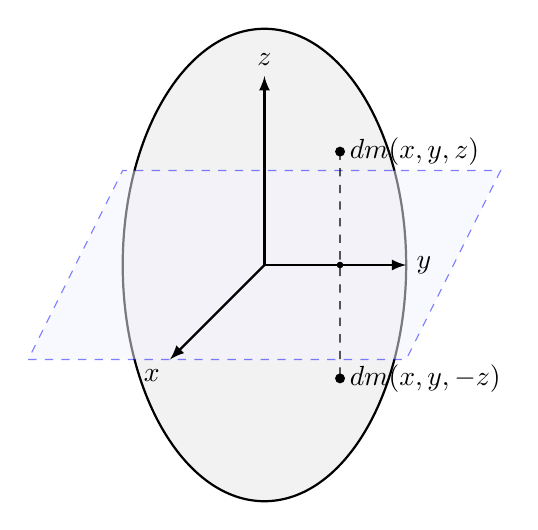
\begin{tikzpicture}[scale=1.2, >=latex]
        % Corpo attraversato dal piano
        \draw[thick, fill=gray!10] (0, 0) ellipse (1.5 and 2.5);
        
        % Piano di simmetria (x,y) in prospettiva
        \draw[dashed, blue, fill=blue!5, opacity=0.5] (-2.5,-1) -- (1.5,-1) -- (2.5,1) -- (-1.5,1) -- cycle;
        
        % Assi
        \draw[->, thick] (0,0) -- (1.5,0) node[right] {$y$};
        \draw[->, thick] (0,0) -- (0,2) node[above] {$z$};
        \draw[->, thick] (0,0) -- (-1,-1) node[below left] {$x$};
        
        % Punti simmetrici
        \coordinate (P1) at (0.8, 1.2);
        \coordinate (P2) at (0.8, -1.2);
        
        \fill (P1) circle (1.5pt) node[right] {$dm(x,y,z)$};
        \fill (P2) circle (1.5pt) node[right] {$dm(x,y,-z)$};
        
        \draw[dashed] (P1) -- (0.8,0) -- (P2);
        \fill (0.8,0) circle (1pt);
    \end{tikzpicture}
    \caption{Rappresentazione di un corpo tagliato dal suo piano di simmetria equatoriale.}
\end{figure}

\paragraph{3) Centro di Simmetria}
Se un corpo possiede un \textbf{centro di simmetria}, il suo Centro di Massa coinciderà esattamente con tale punto.
Alcuni esempi notevoli:
\begin{itemize}
    \item \textbf{Sfera omogenea}: Ogni diametro rappresenta un asse di simmetria. Il centro geometrico funge da centro di simmetria ed è anche il Centro di Massa. In questo caso, il CM appartiene materialmente al corpo ($CM \in \text{corpo}$).
    \item \textbf{Superficie sferica (guscio)}: Valgono le stesse considerazioni di simmetria della sfera piena, ma in questo caso il CM si trova nel vuoto al centro della bolla ($CM \notin \text{corpo}$).
    \item \textbf{Cilindro omogeneo}: L'asse longitudinale è l'asse di simmetria. Inoltre possiede un piano di simmetria trasversale a metà altezza ($h/2$). Il CM giace all'intersezione tra l'asse del cilindro e il piano di simmetria.
\end{itemize}

\section{Forza Totale, Momento Totale e Baricentro}
Per un corpo esteso immerso in un campo gravitazionale $\vec{g}$, la forza agente su un elemento di massa infinitesimo $dm$ è $d\vec{F} = dm \, \vec{g}(dm)$. La \textbf{forza totale} si ottiene integrando su tutto il volume del corpo:
\begin{equation}
    \vec{F}_{tot} = \int_{CR} dm \, \vec{g}(dm)
\end{equation}

Nel caso tipico in cui le dimensioni del corpo siano del tutto trascurabili rispetto al raggio terrestre ($d \ll R_{\text{terra}}$), l'accelerazione di gravità si può considerare \textbf{costante} su tutta l'estensione del corpo ($\vec{g} = \text{costante}$). In tal caso, il vettore $\vec{g}$ può essere portato fuori dall'integrale:
\begin{equation}
    \vec{F}_{tot} = \vec{g} \int_{CR} dm = M \vec{g}
\end{equation}
(In generale, per corpi estremamente estesi come le montagne o interi continenti, l'approssimazione di $\vec{g}$ costante non è più valida e bisogna integrare tenendo conto del gradiente gravitazionale locale).

\subsection{Definizione di Baricentro}
A quale punto geometrico si può immaginare applicata la forza totale $\vec{F}_{tot}$ in modo che eserciti lo stesso momento torcente generato dalla somma di tutti i pesi infinitesimi? Questo punto si chiama \textbf{baricentro}.

Sia $d\vec{F} = \vec{g} \, dm$. Il momento torcente infinitesimo generato da questa forza rispetto al polo di rotazione $O$ è:
\begin{equation}
    d\vec{\tau}_O = \vec{R}(dm) \times d\vec{F}(dm) = dm \, (\vec{R} \times \vec{g})
\end{equation}
Integrando su tutto il corpo rigido, il momento totale risulta:
\begin{equation}
    \vec{\tau}_O = \int_{CR} d\vec{\tau}_O = \int_{CR} dm \, (\vec{R} \times \vec{g})
\end{equation}

Sotto l'ipotesi in cui l'accelerazione di gravità sia rigorosamente costante su tutto il volume, si può estrarre il prodotto vettoriale per $\vec{g}$ fuori dall'integrale:
\begin{equation}
    \vec{\tau}_O = \left( \int_{CR} dm \, \vec{R} \right) \times \vec{g} = (M \vec{R}_{CM}) \times \vec{g} = \vec{R}_{CM} \times (M \vec{g}) = \vec{R}_{CM} \times \vec{F}_{tot}
\end{equation}

Questa relazione fondamentale dimostra che, se $\vec{g}$ è costante, il momento totale generato dalla gravità su un corpo esteso equivale al momento della sola forza totale $M\vec{g}$ \textbf{applicata nel Centro di Massa} ($\vec{R}_{CM}$). 

Ne consegue che \textbf{il baricentro (centro di gravità) e il centro di massa coincidono}, ma \textit{solo} nell'approssimazione di un campo gravitazionale uniforme.
\begin{osservazione}{}
L'omogeneità o disomogeneità della densità del corpo non invalida questa coincidenza: fintantoché $\vec{g}$ è costante, CM e Baricentro saranno sempre lo stesso punto.
\end{osservazione}
